% Copyright 2004 by Till Tantau <tantau@users.sourceforge.net>.
%
% In principle, this file can be redistributed and/or modified under
% the terms of the GNU Public License, version 2.
%
% However, this file is supposed to be a template to be modified
% for your own needs. For this reason, if you use this file as a
% template and not specifically distribute it as part of a another
% package/program, I grant the extra permission to freely copy and
% modify this file as you see fit and even to delete this copyright
% notice. 
\documentclass{beamer}
\usepackage[croatian]{babel}
\usepackage[utf8]{inputenc}
\usepackage{subfig}
\usepackage{booktabs}
\usepackage{multirow}
\usepackage{url}
\usepackage[T1]{fontenc}
\usepackage{caption}
\usepackage{tabularx}
\usepackage{array}
\usepackage{float}
\usepackage{algpseudocode}
\usepackage{algorithm}
\usepackage{pgfplots}

% There are many different themes available for Beamer. A comprehensive
% list with examples is given here:
% http://deic.uab.es/~iblanes/beamer_gallery/index_by_theme.html
% You can uncomment the themes below if you would like to use a different
% one:
%\usetheme{AnnArbor}
%\usetheme{Antibes}
%\usetheme{Bergen}
%\usetheme{Berkeley}
%\usetheme{Berlin}
%\usetheme{Boadilla}
%\usetheme{boxes}
%\usetheme{CambridgeUS}
%\usetheme{Copenhagen}
%\usetheme{Darmstadt}
%\usetheme{default}
%\usetheme{Frankfurt}
%\usetheme{Goettingen}
%\usetheme{Hannover}
%\usetheme{Ilmenau}
%\usetheme{JuanLesPins}
%\usetheme{Luebeck}
\usetheme{Madrid}
%\usetheme{Malmoe}
%\usetheme{Marburg}
%\usetheme{Montpellier}
%\usetheme{PaloAlto}
%\usetheme{Pittsburgh}
%\usetheme{Rochester}
%\usetheme{Singapore}
%\usetheme{Szeged}
%\usetheme{Warsaw}

\makeatletter
\newcommand\titlegraphicii[1]{\def\inserttitlegraphicii{#1}}
\titlegraphicii{}
\setbeamertemplate{title page}
{
  \vbox{}
   {\usebeamercolor[fg]{titlegraphic}\inserttitlegraphic\hfill\inserttitlegraphicii\par}
  \begin{centering}
    \begin{beamercolorbox}[sep=8pt,center]{institute}
      \usebeamerfont{institute}\insertinstitute
    \end{beamercolorbox}
    \begin{beamercolorbox}[sep=8pt,center]{title}
      \ifx\insertsubtitle\@empty%
      \else%
        \vskip0.25em%
        {\usebeamerfont{subtitle}\usebeamercolor[fg]{subtitle}\insertsubtitle\par}%
      \fi%     
        \usebeamerfont{title}\inserttitle\par%
    \end{beamercolorbox}%
    \vskip1em\par
        \begin{beamercolorbox}[sep=8pt,center]{author}
      \usebeamerfont{author}\insertauthor
    \end{beamercolorbox}
    \begin{beamercolorbox}[sep=8pt,center]{date}
      \usebeamerfont{date}\insertdate
    \end{beamercolorbox}%\vskip0.5em
  \end{centering}
  %\vfill
} 
\makeatother
\author{Jure Čular, Bartol Freškura, Filip Gulan}
\title{Izgradnja binarnog stabla valića kao RRR strukture}
\subtitle{Bioinformatika - projekt}
\institute[FER]{Sveučilište u Zagrebu \\ Fakultet elektrotehnike i računarstva}
\date{Zagreb, siječanj 2018.}

 \pgfdeclareimage[height=0.5cm]{university-logo}{logo}
 \logo{\pgfuseimage{university-logo}}

% Let's get started
\begin{document}

\begin{frame}
\maketitle
\end{frame}


% Section and subsections will appear in the presentation overview
% and table of contents.

\section{Uvod}
\begin{frame}{Uvod}
  \begin{itemize}
      \item {
        Sekvence znakova velikih duljina.
      }
      \item{
        Uporaba: potrebno obraditi ili izvršavati određene upite,
      }
      \item{
        Slijedno obrađivanje vrlo sporo.
      }
      \item{
        Rješenje: Binarno stablo valića kao RRR struktura
      }
  \end{itemize}
\end{frame}

\section{RRR struktura}
\subsection{Opis}

\begin{frame}{RRR struktura}{Opis}
  \begin{itemize}
  \item {
    Struktura podatka za pohranjivanje bit-vektora.
  }
  \end{itemize}
     \begin{figure}[H]
    \centering
    \includegraphics[width=0.6\textwidth]{img/superblocks.pdf}
    \caption{Bit vektor podijeljen na blokove i superblokove}
    \end{figure}
    \begin{figure}[H]
    \centering
    \includegraphics[width=0.6\textwidth]{img/coded.pdf}
    \caption{RRR struktura}
    \end{figure}

\end{frame}

\begin{frame}{RRR struktura}{Opis}
  \begin{itemize}
  \item {
    RRR tablicu stvaramo pri kreiranju RRR struktura, pomoću nje izvodimo upite
  }
  \end{itemize}
    \begin{figure}[H]
    \centering
    \includegraphics[height=6cm]{img/rrrtable.png}
    \caption{RRR struktura}
    \end{figure}
\end{frame}

\section{Stablo valića}
\subsection{Opis}
\begin{frame}{Stablo valića}{Opis}
\begin{itemize}
  \item {
    Binarno stablo.
  }
  \item {
    Čvor - podniz ulaznog niza.
  }
    \item {
    Predstavljanje jako dugih sekvenci.
  }
    \item {
    Obavljanje brzih rang upita.
  }
  \end{itemize}
\end{frame}

\begin{frame}{Stablo valića}
    \begin{figure}[H]
    \centering
    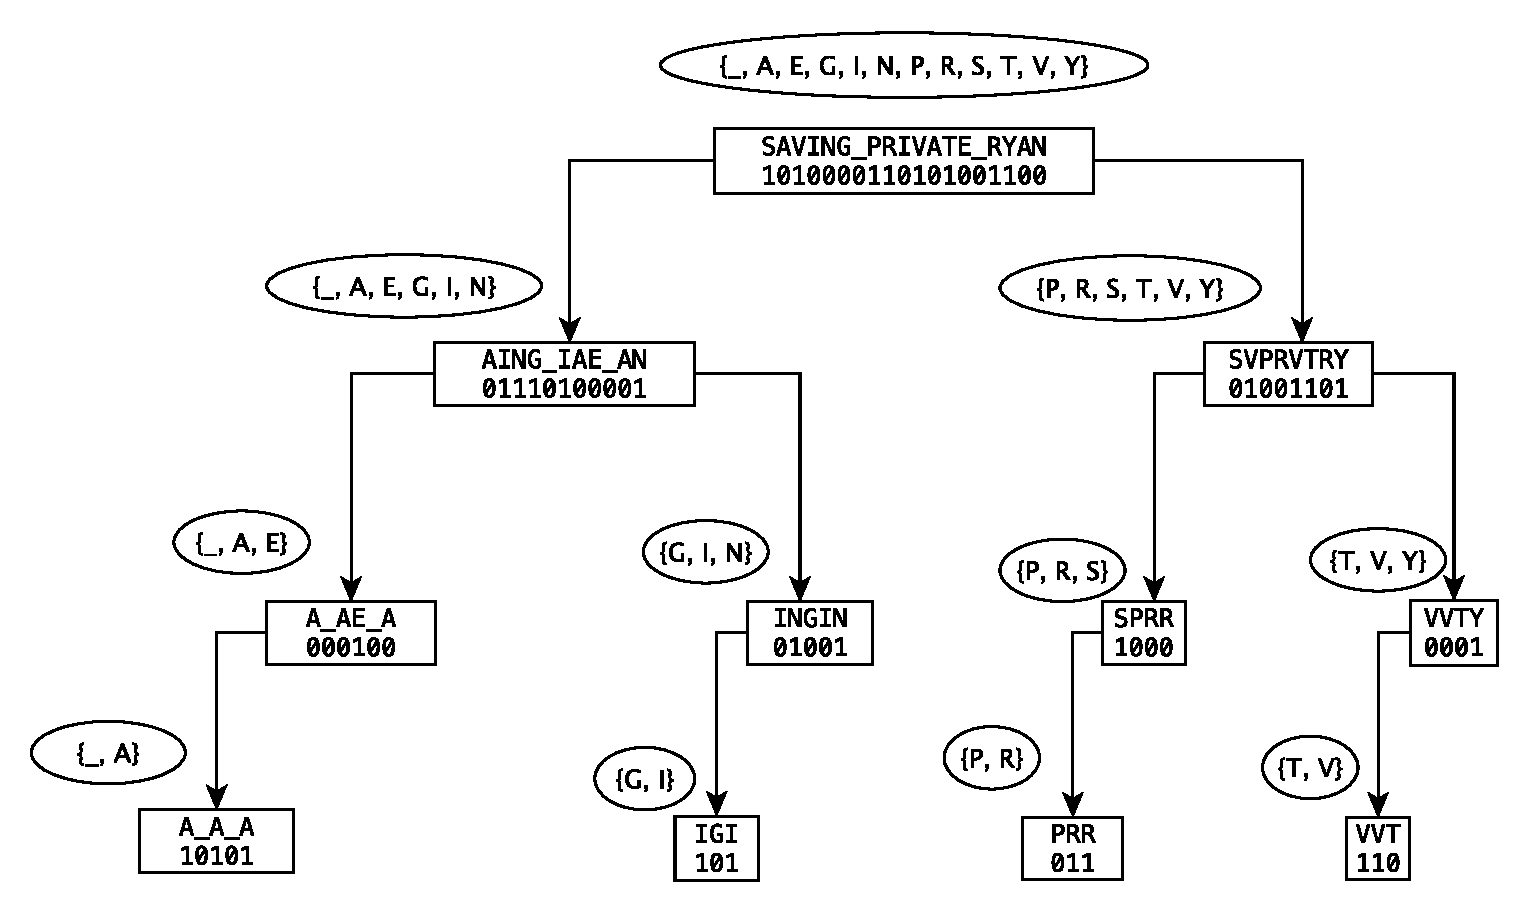
\includegraphics[width=0.9\textwidth]{img/wavelet_tree.pdf}
    \caption{Stablo valića}
    \end{figure}
\end{frame}

\section{Testiranje i rezultati}
\subsection{Stvarni podaci}
\begin{frame}{Rezultati}{Memorija}
\begin{figure}[H]
\centering
\includegraphics[width=0.9\textwidth]{chart/memorija_stabla.png}
\caption{Memorija stabla valić}
\end{figure}
\end{frame}

% \begin{frame}{Rezultati}{Izgradnja stabla}
% \begin{figure}[H]
% \centering
% \includegraphics[width=0.9\textwidth]{chart/vrijeme_izgradnje_stabla.png}
% \caption{Vrijeme izgradnje stabla valić}
% \end{figure}
% \end{frame}

\begin{frame}{Rezultati}{Upiti}
\begin{figure}[H]
\centering
\includegraphics[width=0.9\textwidth]{chart/rank_vrijeme.png}
\caption{Vrijeme rank upita}
\end{figure}
\end{frame}

\begin{frame}{Rezultati}{Upiti}
\begin{figure}[H]
\centering
\includegraphics[width=0.9\textwidth]{chart/vrijeme_select.png}
\caption{Vrijeme select upita}
\end{figure}
\end{frame}

\begin{frame}{Rezultati}{Upiti}
\begin{figure}[H]
\centering
\includegraphics[width=0.9\textwidth]{chart/vrijeme_access.png}
\caption{Vrijeme access upita}
\end{figure}
\end{frame}

\end{document}